\documentclass[twoside]{book}

% Packages required by doxygen
\usepackage{fixltx2e}
\usepackage{calc}
\usepackage{doxygen}
\usepackage[export]{adjustbox} % also loads graphicx
\usepackage{graphicx}
\usepackage[utf8]{inputenc}
\usepackage{makeidx}
\usepackage{multicol}
\usepackage{multirow}
\PassOptionsToPackage{warn}{textcomp}
\usepackage{textcomp}
\usepackage[nointegrals]{wasysym}
\usepackage[table]{xcolor}

% Font selection
\usepackage[T1]{fontenc}
\usepackage[scaled=.90]{helvet}
\usepackage{courier}
\usepackage{amssymb}
\usepackage{sectsty}
\renewcommand{\familydefault}{\sfdefault}
\allsectionsfont{%
  \fontseries{bc}\selectfont%
  \color{darkgray}%
}
\renewcommand{\DoxyLabelFont}{%
  \fontseries{bc}\selectfont%
  \color{darkgray}%
}
\newcommand{\+}{\discretionary{\mbox{\scriptsize$\hookleftarrow$}}{}{}}

% Page & text layout
\usepackage{geometry}
\geometry{%
  a4paper,%
  top=2.5cm,%
  bottom=2.5cm,%
  left=2.5cm,%
  right=2.5cm%
}
\tolerance=750
\hfuzz=15pt
\hbadness=750
\setlength{\emergencystretch}{15pt}
\setlength{\parindent}{0cm}
\setlength{\parskip}{3ex plus 2ex minus 2ex}
\makeatletter
\renewcommand{\paragraph}{%
  \@startsection{paragraph}{4}{0ex}{-1.0ex}{1.0ex}{%
    \normalfont\normalsize\bfseries\SS@parafont%
  }%
}
\renewcommand{\subparagraph}{%
  \@startsection{subparagraph}{5}{0ex}{-1.0ex}{1.0ex}{%
    \normalfont\normalsize\bfseries\SS@subparafont%
  }%
}
\makeatother

% Headers & footers
\usepackage{fancyhdr}
\pagestyle{fancyplain}
\fancyhead[LE]{\fancyplain{}{\bfseries\thepage}}
\fancyhead[CE]{\fancyplain{}{}}
\fancyhead[RE]{\fancyplain{}{\bfseries\leftmark}}
\fancyhead[LO]{\fancyplain{}{\bfseries\rightmark}}
\fancyhead[CO]{\fancyplain{}{}}
\fancyhead[RO]{\fancyplain{}{\bfseries\thepage}}
\fancyfoot[LE]{\fancyplain{}{}}
\fancyfoot[CE]{\fancyplain{}{}}
\fancyfoot[RE]{\fancyplain{}{\bfseries\scriptsize Generated by Doxygen }}
\fancyfoot[LO]{\fancyplain{}{\bfseries\scriptsize Generated by Doxygen }}
\fancyfoot[CO]{\fancyplain{}{}}
\fancyfoot[RO]{\fancyplain{}{}}
\renewcommand{\footrulewidth}{0.4pt}
\renewcommand{\chaptermark}[1]{%
  \markboth{#1}{}%
}
\renewcommand{\sectionmark}[1]{%
  \markright{\thesection\ #1}%
}

% Indices & bibliography
\usepackage{natbib}
\usepackage[titles]{tocloft}
\setcounter{tocdepth}{3}
\setcounter{secnumdepth}{5}
\makeindex

% Hyperlinks (required, but should be loaded last)
\usepackage{ifpdf}
\ifpdf
  \usepackage[pdftex,pagebackref=true]{hyperref}
\else
  \usepackage[ps2pdf,pagebackref=true]{hyperref}
\fi
\hypersetup{%
  colorlinks=true,%
  linkcolor=blue,%
  citecolor=blue,%
  unicode%
}

% Custom commands
\newcommand{\clearemptydoublepage}{%
  \newpage{\pagestyle{empty}\cleardoublepage}%
}

\usepackage{caption}
\captionsetup{labelsep=space,justification=centering,font={bf},singlelinecheck=off,skip=4pt,position=top}

%===== C O N T E N T S =====

\begin{document}

% Titlepage & ToC
\hypersetup{pageanchor=false,
             bookmarksnumbered=true,
             pdfencoding=unicode
            }
\pagenumbering{alph}
\begin{titlepage}
\vspace*{7cm}
\begin{center}%
{\Large Server \\[1ex]\large 1.\+6 }\\
\vspace*{1cm}
{\large Generated by Doxygen 1.8.14}\\
\end{center}
\end{titlepage}
\clearemptydoublepage
\pagenumbering{roman}
\tableofcontents
\clearemptydoublepage
\pagenumbering{arabic}
\hypersetup{pageanchor=true}

%--- Begin generated contents ---
\chapter{Hierarchical Index}
\section{Class Hierarchy}
This inheritance list is sorted roughly, but not completely, alphabetically\+:\begin{DoxyCompactList}
\item \contentsline{section}{Node}{\pageref{class_node}}{}
\item Q\+Main\+Window\begin{DoxyCompactList}
\item \contentsline{section}{Main\+Window}{\pageref{class_main_window}}{}
\end{DoxyCompactList}
\item Q\+Widget\begin{DoxyCompactList}
\item \contentsline{section}{Form}{\pageref{class_form}}{}
\end{DoxyCompactList}
\item \contentsline{section}{Tree}{\pageref{class_tree}}{}
\end{DoxyCompactList}

\chapter{Class Index}
\section{Class List}
Here are the classes, structs, unions and interfaces with brief descriptions\+:\begin{DoxyCompactList}
\item\contentsline{section}{\mbox{\hyperlink{class_authorize}{Authorize}} }{\pageref{class_authorize}}{}
\item\contentsline{section}{\mbox{\hyperlink{class_main_window}{Main\+Window}} }{\pageref{class_main_window}}{}
\item\contentsline{section}{\mbox{\hyperlink{class_registration}{Registration}} }{\pageref{class_registration}}{}
\item\contentsline{section}{\mbox{\hyperlink{classtask1}{task1}} }{\pageref{classtask1}}{}
\item\contentsline{section}{\mbox{\hyperlink{classtask2}{task2}} }{\pageref{classtask2}}{}
\item\contentsline{section}{\mbox{\hyperlink{classtask3}{task3}} }{\pageref{classtask3}}{}
\item\contentsline{section}{\mbox{\hyperlink{classtask4}{task4}} }{\pageref{classtask4}}{}
\end{DoxyCompactList}

\chapter{File Index}
\section{File List}
Here is a list of all files with brief descriptions\+:\begin{DoxyCompactList}
\item\contentsline{section}{C\+:/\+Q\+T\+T/\+Prufer/\mbox{\hyperlink{form_8cpp}{form.\+cpp}} }{\pageref{form_8cpp}}{}
\item\contentsline{section}{C\+:/\+Q\+T\+T/\+Prufer/\mbox{\hyperlink{form_8h}{form.\+h}} }{\pageref{form_8h}}{}
\item\contentsline{section}{C\+:/\+Q\+T\+T/\+Prufer/\mbox{\hyperlink{main_8cpp}{main.\+cpp}} }{\pageref{main_8cpp}}{}
\item\contentsline{section}{C\+:/\+Q\+T\+T/\+Prufer/\mbox{\hyperlink{mainwindow_8cpp}{mainwindow.\+cpp}} }{\pageref{mainwindow_8cpp}}{}
\item\contentsline{section}{C\+:/\+Q\+T\+T/\+Prufer/\mbox{\hyperlink{mainwindow_8h}{mainwindow.\+h}} }{\pageref{mainwindow_8h}}{}
\item\contentsline{section}{C\+:/\+Q\+T\+T/\+Prufer/\mbox{\hyperlink{node_8cpp}{node.\+cpp}} }{\pageref{node_8cpp}}{}
\item\contentsline{section}{C\+:/\+Q\+T\+T/\+Prufer/\mbox{\hyperlink{node_8h}{node.\+h}} }{\pageref{node_8h}}{}
\item\contentsline{section}{C\+:/\+Q\+T\+T/\+Prufer/\mbox{\hyperlink{tree_8cpp}{tree.\+cpp}} }{\pageref{tree_8cpp}}{}
\item\contentsline{section}{C\+:/\+Q\+T\+T/\+Prufer/\mbox{\hyperlink{tree_8h}{tree.\+h}} }{\pageref{tree_8h}}{}
\end{DoxyCompactList}

\chapter{Class Documentation}
\hypertarget{class_data_base}{}\section{Data\+Base Class Reference}
\label{class_data_base}\index{Data\+Base@{Data\+Base}}


{\ttfamily \#include $<$database.\+h$>$}

\subsection*{Public Member Functions}
\begin{DoxyCompactItemize}
\item 
void \mbox{\hyperlink{class_data_base_adb17c56e22c3fe77bbd682bee8811a56}{close\+DB}} ()
\end{DoxyCompactItemize}
\subsection*{Static Public Member Functions}
\begin{DoxyCompactItemize}
\item 
static \mbox{\hyperlink{class_data_base}{Data\+Base}} $\ast$ \mbox{\hyperlink{class_data_base_abe2f75c0d6067414a1fbb22dc166ca46}{get\+Instance}} ()
\item 
static Q\+Byte\+Array \mbox{\hyperlink{class_data_base_a0f8839a75f6881d6b4a9e7d3eed0fb78}{test}} ()
\end{DoxyCompactItemize}
\subsection*{Protected Member Functions}
\begin{DoxyCompactItemize}
\item 
\mbox{\hyperlink{class_data_base_a9fbd4936704ce4de391f92e92a072074}{Data\+Base}} ()
\item 
\mbox{\hyperlink{class_data_base_aebdd1dfd170fef81ff0365609d63e533}{Data\+Base}} (const \mbox{\hyperlink{class_data_base}{Data\+Base}} \&)
\item 
\mbox{\hyperlink{class_data_base}{Data\+Base}} \& \mbox{\hyperlink{class_data_base_ac5c47c845425deafd990f249077297ab}{operator=}} (\mbox{\hyperlink{class_data_base}{Data\+Base}} \&)
\item 
\mbox{\hyperlink{class_data_base_a9d4629e705ccaa4897e9650222a2a648}{$\sim$\+Data\+Base}} ()
\end{DoxyCompactItemize}
\subsection*{Friends}
\begin{DoxyCompactItemize}
\item 
class \mbox{\hyperlink{class_data_base_a2de1189b514a6e1f7c31c180dc27f000}{Data\+Base\+Destroyer}}
\end{DoxyCompactItemize}


\subsection{Constructor \& Destructor Documentation}
\mbox{\Hypertarget{class_data_base_a9fbd4936704ce4de391f92e92a072074}\label{class_data_base_a9fbd4936704ce4de391f92e92a072074}} 
\index{Data\+Base@{Data\+Base}!Data\+Base@{Data\+Base}}
\index{Data\+Base@{Data\+Base}!Data\+Base@{Data\+Base}}
\subsubsection{\texorpdfstring{Data\+Base()}{DataBase()}\hspace{0.1cm}{\footnotesize\ttfamily [1/2]}}
{\footnotesize\ttfamily Data\+Base\+::\+Data\+Base (\begin{DoxyParamCaption}{ }\end{DoxyParamCaption})\hspace{0.3cm}{\ttfamily [protected]}}

\mbox{\Hypertarget{class_data_base_aebdd1dfd170fef81ff0365609d63e533}\label{class_data_base_aebdd1dfd170fef81ff0365609d63e533}} 
\index{Data\+Base@{Data\+Base}!Data\+Base@{Data\+Base}}
\index{Data\+Base@{Data\+Base}!Data\+Base@{Data\+Base}}
\subsubsection{\texorpdfstring{Data\+Base()}{DataBase()}\hspace{0.1cm}{\footnotesize\ttfamily [2/2]}}
{\footnotesize\ttfamily Data\+Base\+::\+Data\+Base (\begin{DoxyParamCaption}\item[{const \mbox{\hyperlink{class_data_base}{Data\+Base}} \&}]{ }\end{DoxyParamCaption})\hspace{0.3cm}{\ttfamily [protected]}}

\mbox{\Hypertarget{class_data_base_a9d4629e705ccaa4897e9650222a2a648}\label{class_data_base_a9d4629e705ccaa4897e9650222a2a648}} 
\index{Data\+Base@{Data\+Base}!````~Data\+Base@{$\sim$\+Data\+Base}}
\index{````~Data\+Base@{$\sim$\+Data\+Base}!Data\+Base@{Data\+Base}}
\subsubsection{\texorpdfstring{$\sim$\+Data\+Base()}{~DataBase()}}
{\footnotesize\ttfamily Data\+Base\+::$\sim$\+Data\+Base (\begin{DoxyParamCaption}{ }\end{DoxyParamCaption})\hspace{0.3cm}{\ttfamily [inline]}, {\ttfamily [protected]}}



\subsection{Member Function Documentation}
\mbox{\Hypertarget{class_data_base_adb17c56e22c3fe77bbd682bee8811a56}\label{class_data_base_adb17c56e22c3fe77bbd682bee8811a56}} 
\index{Data\+Base@{Data\+Base}!close\+DB@{close\+DB}}
\index{close\+DB@{close\+DB}!Data\+Base@{Data\+Base}}
\subsubsection{\texorpdfstring{close\+D\+B()}{closeDB()}}
{\footnotesize\ttfamily void Data\+Base\+::close\+DB (\begin{DoxyParamCaption}{ }\end{DoxyParamCaption})\hspace{0.3cm}{\ttfamily [inline]}}

\mbox{\Hypertarget{class_data_base_abe2f75c0d6067414a1fbb22dc166ca46}\label{class_data_base_abe2f75c0d6067414a1fbb22dc166ca46}} 
\index{Data\+Base@{Data\+Base}!get\+Instance@{get\+Instance}}
\index{get\+Instance@{get\+Instance}!Data\+Base@{Data\+Base}}
\subsubsection{\texorpdfstring{get\+Instance()}{getInstance()}}
{\footnotesize\ttfamily static \mbox{\hyperlink{class_data_base}{Data\+Base}}$\ast$ Data\+Base\+::get\+Instance (\begin{DoxyParamCaption}{ }\end{DoxyParamCaption})\hspace{0.3cm}{\ttfamily [inline]}, {\ttfamily [static]}}

\mbox{\Hypertarget{class_data_base_ac5c47c845425deafd990f249077297ab}\label{class_data_base_ac5c47c845425deafd990f249077297ab}} 
\index{Data\+Base@{Data\+Base}!operator=@{operator=}}
\index{operator=@{operator=}!Data\+Base@{Data\+Base}}
\subsubsection{\texorpdfstring{operator=()}{operator=()}}
{\footnotesize\ttfamily \mbox{\hyperlink{class_data_base}{Data\+Base}}\& Data\+Base\+::operator= (\begin{DoxyParamCaption}\item[{\mbox{\hyperlink{class_data_base}{Data\+Base}} \&}]{ }\end{DoxyParamCaption})\hspace{0.3cm}{\ttfamily [protected]}}

\mbox{\Hypertarget{class_data_base_a0f8839a75f6881d6b4a9e7d3eed0fb78}\label{class_data_base_a0f8839a75f6881d6b4a9e7d3eed0fb78}} 
\index{Data\+Base@{Data\+Base}!test@{test}}
\index{test@{test}!Data\+Base@{Data\+Base}}
\subsubsection{\texorpdfstring{test()}{test()}}
{\footnotesize\ttfamily static Q\+Byte\+Array Data\+Base\+::test (\begin{DoxyParamCaption}{ }\end{DoxyParamCaption})\hspace{0.3cm}{\ttfamily [inline]}, {\ttfamily [static]}}



\subsection{Friends And Related Function Documentation}
\mbox{\Hypertarget{class_data_base_a2de1189b514a6e1f7c31c180dc27f000}\label{class_data_base_a2de1189b514a6e1f7c31c180dc27f000}} 
\index{Data\+Base@{Data\+Base}!Data\+Base\+Destroyer@{Data\+Base\+Destroyer}}
\index{Data\+Base\+Destroyer@{Data\+Base\+Destroyer}!Data\+Base@{Data\+Base}}
\subsubsection{\texorpdfstring{Data\+Base\+Destroyer}{DataBaseDestroyer}}
{\footnotesize\ttfamily friend class \mbox{\hyperlink{class_data_base_destroyer}{Data\+Base\+Destroyer}}\hspace{0.3cm}{\ttfamily [friend]}}



The documentation for this class was generated from the following files\+:\begin{DoxyCompactItemize}
\item 
C\+:/\+Q\+T\+T/\+Sborka/server/\mbox{\hyperlink{database_8h}{database.\+h}}\item 
C\+:/\+Q\+T\+T/\+Sborka/server/\mbox{\hyperlink{database_8cpp}{database.\+cpp}}\end{DoxyCompactItemize}

\hypertarget{class_data_base_destroyer}{}\section{Data\+Base\+Destroyer Class Reference}
\label{class_data_base_destroyer}\index{Data\+Base\+Destroyer@{Data\+Base\+Destroyer}}


{\ttfamily \#include $<$database.\+h$>$}

\subsection*{Public Member Functions}
\begin{DoxyCompactItemize}
\item 
\mbox{\hyperlink{class_data_base_destroyer_a2be0488f65d1495e0e303efb01013e62}{$\sim$\+Data\+Base\+Destroyer}} ()
\item 
void \mbox{\hyperlink{class_data_base_destroyer_aee85b804dca5015f185f2c1b47d85aa3}{initialize}} (\mbox{\hyperlink{class_data_base}{Data\+Base}} $\ast$p)
\end{DoxyCompactItemize}


\subsection{Constructor \& Destructor Documentation}
\mbox{\Hypertarget{class_data_base_destroyer_a2be0488f65d1495e0e303efb01013e62}\label{class_data_base_destroyer_a2be0488f65d1495e0e303efb01013e62}} 
\index{Data\+Base\+Destroyer@{Data\+Base\+Destroyer}!````~Data\+Base\+Destroyer@{$\sim$\+Data\+Base\+Destroyer}}
\index{````~Data\+Base\+Destroyer@{$\sim$\+Data\+Base\+Destroyer}!Data\+Base\+Destroyer@{Data\+Base\+Destroyer}}
\subsubsection{\texorpdfstring{$\sim$\+Data\+Base\+Destroyer()}{~DataBaseDestroyer()}}
{\footnotesize\ttfamily Data\+Base\+Destroyer\+::$\sim$\+Data\+Base\+Destroyer (\begin{DoxyParamCaption}{ }\end{DoxyParamCaption})\hspace{0.3cm}{\ttfamily [inline]}}



\subsection{Member Function Documentation}
\mbox{\Hypertarget{class_data_base_destroyer_aee85b804dca5015f185f2c1b47d85aa3}\label{class_data_base_destroyer_aee85b804dca5015f185f2c1b47d85aa3}} 
\index{Data\+Base\+Destroyer@{Data\+Base\+Destroyer}!initialize@{initialize}}
\index{initialize@{initialize}!Data\+Base\+Destroyer@{Data\+Base\+Destroyer}}
\subsubsection{\texorpdfstring{initialize()}{initialize()}}
{\footnotesize\ttfamily void Data\+Base\+Destroyer\+::initialize (\begin{DoxyParamCaption}\item[{\mbox{\hyperlink{class_data_base}{Data\+Base}} $\ast$}]{p }\end{DoxyParamCaption})\hspace{0.3cm}{\ttfamily [inline]}}



The documentation for this class was generated from the following file\+:\begin{DoxyCompactItemize}
\item 
C\+:/\+Q\+T\+T/\+Sborka/server/\mbox{\hyperlink{database_8h}{database.\+h}}\end{DoxyCompactItemize}

\hypertarget{class_my_tcp_server}{}\doxysection{My\+Tcp\+Server Class Reference}
\label{class_my_tcp_server}\index{MyTcpServer@{MyTcpServer}}


\mbox{\hyperlink{class_my_tcp_server}{My\+Tcp\+Server}} -\/ класс сервера, содержащий начальные настройки  




{\ttfamily \#include $<$mytcpserver.\+h$>$}

Inheritance diagram for My\+Tcp\+Server\+:\begin{figure}[H]
\begin{center}
\leavevmode
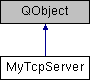
\includegraphics[height=2.000000cm]{class_my_tcp_server}
\end{center}
\end{figure}
\doxysubsection*{Public Slots}
\begin{DoxyCompactItemize}
\item 
void \mbox{\hyperlink{class_my_tcp_server_a0ba7316ffe1a26c57fabde9e74b6c8dc}{slot\+New\+Connection}} ()
\begin{DoxyCompactList}\small\item\em Слот нового подключения \end{DoxyCompactList}\item 
void \mbox{\hyperlink{class_my_tcp_server_a3e040c49dbefd65b9a58ab662fc9f7a2}{slot\+Client\+Disconnected}} ()
\begin{DoxyCompactList}\small\item\em Слот отключения \end{DoxyCompactList}\item 
void \mbox{\hyperlink{class_my_tcp_server_ab4a64d2eab985d723090963f5c8a2882}{slot\+Server\+Read}} ()
\begin{DoxyCompactList}\small\item\em Слот чтения \end{DoxyCompactList}\end{DoxyCompactItemize}
\doxysubsection*{Public Member Functions}
\begin{DoxyCompactItemize}
\item 
\mbox{\hyperlink{class_my_tcp_server_acf367c4695b4d160c7a2d25c2afaaec4}{My\+Tcp\+Server}} (QObject $\ast$parent=nullptr)
\begin{DoxyCompactList}\small\item\em Конструктор объекта сервера \end{DoxyCompactList}\item 
\mbox{\Hypertarget{class_my_tcp_server_ab39e651ff7c37c152215c02c225e79ef}\label{class_my_tcp_server_ab39e651ff7c37c152215c02c225e79ef}} 
{\bfseries $\sim$\+My\+Tcp\+Server} ()
\begin{DoxyCompactList}\small\item\em Деструктор объекта сервера \end{DoxyCompactList}\end{DoxyCompactItemize}


\doxysubsection{Detailed Description}
\mbox{\hyperlink{class_my_tcp_server}{My\+Tcp\+Server}} -\/ класс сервера, содержащий начальные настройки 

В этом классе объявлены слоты для обработки подключения, отключения клиентов и обработки ввода пользователей \mbox{\hyperlink{class_my_tcp_server_a0ba7316ffe1a26c57fabde9e74b6c8dc}{slot\+New\+Connection()}} -\/ слот для обработки нового подключения \mbox{\hyperlink{class_my_tcp_server_a3e040c49dbefd65b9a58ab662fc9f7a2}{slot\+Client\+Disconnected()}} -\/ слот для обработки отключения клиента \mbox{\hyperlink{class_my_tcp_server_ab4a64d2eab985d723090963f5c8a2882}{slot\+Server\+Read()}} -\/ слот для обработки ввода клиентов 

\doxysubsection{Constructor \& Destructor Documentation}
\mbox{\Hypertarget{class_my_tcp_server_acf367c4695b4d160c7a2d25c2afaaec4}\label{class_my_tcp_server_acf367c4695b4d160c7a2d25c2afaaec4}} 
\index{MyTcpServer@{MyTcpServer}!MyTcpServer@{MyTcpServer}}
\index{MyTcpServer@{MyTcpServer}!MyTcpServer@{MyTcpServer}}
\doxysubsubsection{\texorpdfstring{MyTcpServer()}{MyTcpServer()}}
{\footnotesize\ttfamily My\+Tcp\+Server\+::\+My\+Tcp\+Server (\begin{DoxyParamCaption}\item[{QObject $\ast$}]{parent = {\ttfamily nullptr} }\end{DoxyParamCaption})\hspace{0.3cm}{\ttfamily [explicit]}}



Конструктор объекта сервера 

Производит инициализацию объекта сервера с уведомлением о статусе сервера 

\doxysubsection{Member Function Documentation}
\mbox{\Hypertarget{class_my_tcp_server_a3e040c49dbefd65b9a58ab662fc9f7a2}\label{class_my_tcp_server_a3e040c49dbefd65b9a58ab662fc9f7a2}} 
\index{MyTcpServer@{MyTcpServer}!slotClientDisconnected@{slotClientDisconnected}}
\index{slotClientDisconnected@{slotClientDisconnected}!MyTcpServer@{MyTcpServer}}
\doxysubsubsection{\texorpdfstring{slotClientDisconnected}{slotClientDisconnected}}
{\footnotesize\ttfamily void My\+Tcp\+Server\+::slot\+Client\+Disconnected (\begin{DoxyParamCaption}{ }\end{DoxyParamCaption})\hspace{0.3cm}{\ttfamily [slot]}}



Слот отключения 

Удаляет сокета из списка клиентов и закрывает его \mbox{\Hypertarget{class_my_tcp_server_a0ba7316ffe1a26c57fabde9e74b6c8dc}\label{class_my_tcp_server_a0ba7316ffe1a26c57fabde9e74b6c8dc}} 
\index{MyTcpServer@{MyTcpServer}!slotNewConnection@{slotNewConnection}}
\index{slotNewConnection@{slotNewConnection}!MyTcpServer@{MyTcpServer}}
\doxysubsubsection{\texorpdfstring{slotNewConnection}{slotNewConnection}}
{\footnotesize\ttfamily void My\+Tcp\+Server\+::slot\+New\+Connection (\begin{DoxyParamCaption}{ }\end{DoxyParamCaption})\hspace{0.3cm}{\ttfamily [slot]}}



Слот нового подключения 

Создаёт новый объект сокета, инициализирует его и производит запись в список клиентов \mbox{\Hypertarget{class_my_tcp_server_ab4a64d2eab985d723090963f5c8a2882}\label{class_my_tcp_server_ab4a64d2eab985d723090963f5c8a2882}} 
\index{MyTcpServer@{MyTcpServer}!slotServerRead@{slotServerRead}}
\index{slotServerRead@{slotServerRead}!MyTcpServer@{MyTcpServer}}
\doxysubsubsection{\texorpdfstring{slotServerRead}{slotServerRead}}
{\footnotesize\ttfamily void My\+Tcp\+Server\+::slot\+Server\+Read (\begin{DoxyParamCaption}{ }\end{DoxyParamCaption})\hspace{0.3cm}{\ttfamily [slot]}}



Слот чтения 

Считывает пользовательский ввод и передаёт данные в функцию парсинга 

The documentation for this class was generated from the following files\+:\begin{DoxyCompactItemize}
\item 
D\+:/echo\+Server/\+PTechnologies/mytcpserver.\+h\item 
D\+:/echo\+Server/\+PTechnologies/mytcpserver.\+cpp\end{DoxyCompactItemize}

\chapter{File Documentation}
\hypertarget{database_8cpp}{}\section{C\+:/\+Q\+T\+T/\+Sborka/server/database.cpp File Reference}
\label{database_8cpp}\index{C\+:/\+Q\+T\+T/\+Sborka/server/database.\+cpp@{C\+:/\+Q\+T\+T/\+Sborka/server/database.\+cpp}}
{\ttfamily \#include \char`\"{}database.\+h\char`\"{}}\newline
Include dependency graph for database.\+cpp\+:

\hypertarget{database_8h}{}\section{C\+:/\+Q\+T\+T/\+Sborka/server/database.h File Reference}
\label{database_8h}\index{C\+:/\+Q\+T\+T/\+Sborka/server/database.\+h@{C\+:/\+Q\+T\+T/\+Sborka/server/database.\+h}}
{\ttfamily \#include $<$Q\+Debug$>$}\newline
{\ttfamily \#include $<$Q\+Sql\+Database$>$}\newline
{\ttfamily \#include $<$Q\+Sql\+Query$>$}\newline
{\ttfamily \#include $<$Q\+Sql\+Error$>$}\newline
{\ttfamily \#include $<$Q\+Sql\+Record$>$}\newline
Include dependency graph for database.\+h\+:
% FIG 0
This graph shows which files directly or indirectly include this file\+:
% FIG 1
\subsection*{Classes}
\begin{DoxyCompactItemize}
\item 
class \mbox{\hyperlink{class_data_base_destroyer}{Data\+Base\+Destroyer}}
\item 
class \mbox{\hyperlink{class_data_base}{Data\+Base}}
\end{DoxyCompactItemize}

\hypertarget{functionsforserver_8cpp}{}\section{C\+:/\+Q\+T\+T/\+Sborka/server/functionsforserver.cpp File Reference}
\label{functionsforserver_8cpp}\index{C\+:/\+Q\+T\+T/\+Sborka/server/functionsforserver.\+cpp@{C\+:/\+Q\+T\+T/\+Sborka/server/functionsforserver.\+cpp}}
{\ttfamily \#include \char`\"{}functionsforserver.\+h\char`\"{}}\newline
{\ttfamily \#include \char`\"{}database.\+h\char`\"{}}\newline
{\ttfamily \#include $<$Q\+String\+List$>$}\newline
{\ttfamily \#include $<$Q\+String$>$}\newline
{\ttfamily \#include $<$Q\+Map$>$}\newline
{\ttfamily \#include $<$Q\+Debug$>$}\newline
Include dependency graph for functionsforserver.\+cpp\+:
% FIG 0
\subsection*{Functions}
\begin{DoxyCompactItemize}
\item 
Q\+Byte\+Array \mbox{\hyperlink{functionsforserver_8cpp_a35ec2c03b2fa42dbee1c13e5b89d768c}{auth}} (Q\+String log)
\item 
Q\+Byte\+Array \mbox{\hyperlink{functionsforserver_8cpp_af15516dbde168cd1fabbce8e4209b5a5}{parsing}} (Q\+String data\+\_\+from\+\_\+client)
\end{DoxyCompactItemize}


\subsection{Function Documentation}
\mbox{\Hypertarget{functionsforserver_8cpp_a35ec2c03b2fa42dbee1c13e5b89d768c}\label{functionsforserver_8cpp_a35ec2c03b2fa42dbee1c13e5b89d768c}} 
\index{functionsforserver.\+cpp@{functionsforserver.\+cpp}!auth@{auth}}
\index{auth@{auth}!functionsforserver.\+cpp@{functionsforserver.\+cpp}}
\subsubsection{\texorpdfstring{auth()}{auth()}}
{\footnotesize\ttfamily Q\+Byte\+Array auth (\begin{DoxyParamCaption}\item[{Q\+String}]{log }\end{DoxyParamCaption})}

\mbox{\Hypertarget{functionsforserver_8cpp_af15516dbde168cd1fabbce8e4209b5a5}\label{functionsforserver_8cpp_af15516dbde168cd1fabbce8e4209b5a5}} 
\index{functionsforserver.\+cpp@{functionsforserver.\+cpp}!parsing@{parsing}}
\index{parsing@{parsing}!functionsforserver.\+cpp@{functionsforserver.\+cpp}}
\subsubsection{\texorpdfstring{parsing()}{parsing()}}
{\footnotesize\ttfamily Q\+Byte\+Array parsing (\begin{DoxyParamCaption}\item[{Q\+String}]{data\+\_\+from\+\_\+client }\end{DoxyParamCaption})}


\hypertarget{functionsforserver_8h}{}\section{C\+:/\+Q\+T\+T/\+Sborka/server/functionsforserver.h File Reference}
\label{functionsforserver_8h}\index{C\+:/\+Q\+T\+T/\+Sborka/server/functionsforserver.\+h@{C\+:/\+Q\+T\+T/\+Sborka/server/functionsforserver.\+h}}
{\ttfamily \#include $<$Q\+String$>$}\newline
Include dependency graph for functionsforserver.\+h\+:
% FIG 0
This graph shows which files directly or indirectly include this file\+:
% FIG 1
\subsection*{Functions}
\begin{DoxyCompactItemize}
\item 
Q\+Byte\+Array \mbox{\hyperlink{functionsforserver_8h_af15516dbde168cd1fabbce8e4209b5a5}{parsing}} (Q\+String data\+\_\+from\+\_\+client)
\item 
Q\+Byte\+Array \mbox{\hyperlink{functionsforserver_8h_a35ec2c03b2fa42dbee1c13e5b89d768c}{auth}} (Q\+String log)
\end{DoxyCompactItemize}


\subsection{Function Documentation}
\mbox{\Hypertarget{functionsforserver_8h_a35ec2c03b2fa42dbee1c13e5b89d768c}\label{functionsforserver_8h_a35ec2c03b2fa42dbee1c13e5b89d768c}} 
\index{functionsforserver.\+h@{functionsforserver.\+h}!auth@{auth}}
\index{auth@{auth}!functionsforserver.\+h@{functionsforserver.\+h}}
\subsubsection{\texorpdfstring{auth()}{auth()}}
{\footnotesize\ttfamily Q\+Byte\+Array auth (\begin{DoxyParamCaption}\item[{Q\+String}]{log }\end{DoxyParamCaption})}

\mbox{\Hypertarget{functionsforserver_8h_af15516dbde168cd1fabbce8e4209b5a5}\label{functionsforserver_8h_af15516dbde168cd1fabbce8e4209b5a5}} 
\index{functionsforserver.\+h@{functionsforserver.\+h}!parsing@{parsing}}
\index{parsing@{parsing}!functionsforserver.\+h@{functionsforserver.\+h}}
\subsubsection{\texorpdfstring{parsing()}{parsing()}}
{\footnotesize\ttfamily Q\+Byte\+Array parsing (\begin{DoxyParamCaption}\item[{Q\+String}]{data\+\_\+from\+\_\+client }\end{DoxyParamCaption})}


\hypertarget{main_8cpp}{}\section{C\+:/\+Q\+T\+T/\+Sborka/server/main.cpp File Reference}
\label{main_8cpp}\index{C\+:/\+Q\+T\+T/\+Sborka/server/main.\+cpp@{C\+:/\+Q\+T\+T/\+Sborka/server/main.\+cpp}}
{\ttfamily \#include $<$Q\+Core\+Application$>$}\newline
{\ttfamily \#include \char`\"{}mytcpserver.\+h\char`\"{}}\newline
{\ttfamily \#include \char`\"{}database.\+h\char`\"{}}\newline
Include dependency graph for main.\+cpp\+:
% FIG 0

\hypertarget{mytcpserver_8cpp}{}\section{C\+:/\+Q\+T\+T/\+Sborka/server/mytcpserver.cpp File Reference}
\label{mytcpserver_8cpp}\index{C\+:/\+Q\+T\+T/\+Sborka/server/mytcpserver.\+cpp@{C\+:/\+Q\+T\+T/\+Sborka/server/mytcpserver.\+cpp}}
{\ttfamily \#include \char`\"{}mytcpserver.\+h\char`\"{}}\newline
{\ttfamily \#include \char`\"{}functionsforserver.\+h\char`\"{}}\newline
{\ttfamily \#include $<$Q\+Debug$>$}\newline
{\ttfamily \#include $<$Q\+Core\+Application$>$}\newline
Include dependency graph for mytcpserver.\+cpp\+:
% FIG 0

\hypertarget{mytcpserver_8h}{}\section{C\+:/\+Q\+T\+T/\+Sborka/server/mytcpserver.h File Reference}
\label{mytcpserver_8h}\index{C\+:/\+Q\+T\+T/\+Sborka/server/mytcpserver.\+h@{C\+:/\+Q\+T\+T/\+Sborka/server/mytcpserver.\+h}}
{\ttfamily \#include $<$Q\+Object$>$}\newline
{\ttfamily \#include $<$Q\+Tcp\+Server$>$}\newline
{\ttfamily \#include $<$Q\+Tcp\+Socket$>$}\newline
{\ttfamily \#include $<$Qt\+Network$>$}\newline
{\ttfamily \#include $<$Q\+Byte\+Array$>$}\newline
{\ttfamily \#include $<$Q\+Debug$>$}\newline
{\ttfamily \#include $<$list$>$}\newline
{\ttfamily \#include \char`\"{}functionsforserver.\+h\char`\"{}}\newline
Include dependency graph for mytcpserver.\+h\+:
% FIG 0
This graph shows which files directly or indirectly include this file\+:
% FIG 1
\subsection*{Classes}
\begin{DoxyCompactItemize}
\item 
class \mbox{\hyperlink{class_my_tcp_server}{My\+Tcp\+Server}}
\end{DoxyCompactItemize}

%--- End generated contents ---

% Index
\backmatter
\newpage
\phantomsection
\clearemptydoublepage
\addcontentsline{toc}{chapter}{Index}
\printindex

\end{document}
